
\newcommand{\TableNote}{$LEAP$ is the Longitudinal Employment Analysis Program and $CanSynLBD$ is the Canadian synthetic database based on LEAP. Here, we use the 2015 vintage of LEAP and drop the last year observations.}

\subsection{Firm Characteristics}

The CanSynLBD and LEAP generally provide comparable inferences on aggregate means and correlations. For example, Figures \ref{GrossEmploymentPrivate} and \ref{GrossEmploymentManufacturing} show that gross employment levels for each year in the CanSynLBD are very close to those in the LEAP. However, the manufacturing sector shows closer patterns than the private sector.\footnote{The private sector comprises all industries including the manufacturing sector except the public sector  (NAICS 61, 62, and 91)} We find similar results for total payroll (Figures \ref{TotalPayrollPrivate} and  \ref{TotalPayrollManufacturing}) .

\todo{Why is manufacturing always below, but overall employment crosses? Which industries are driving that?} \todo{JA: I checked before, but I could not able to identify any specific reason.}
\begin{figure} [H]
\centering
\caption{Gross employment level by year (private)} \label{GrossEmploymentPrivate}
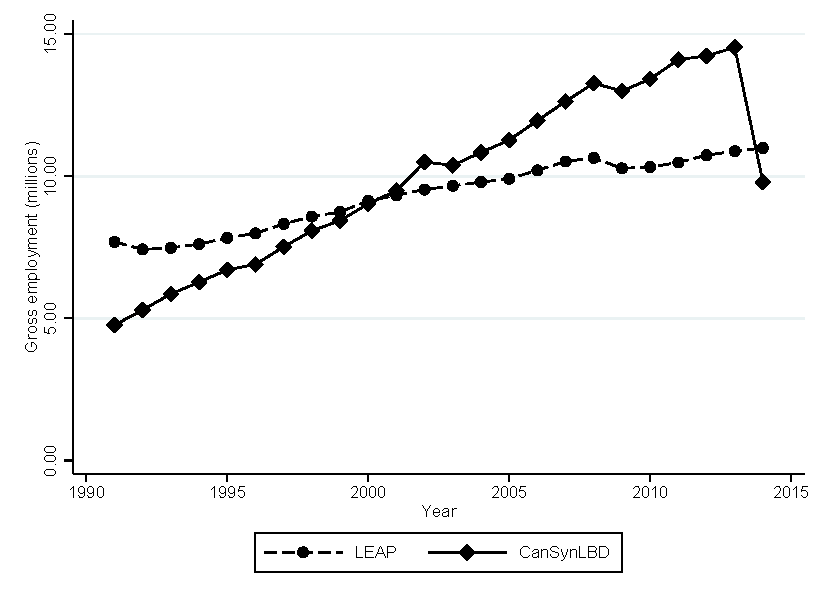
\includegraphics[height=2.8in, width=.7\linewidth]{graphs/Gross_employment_level_by_year_private_bw.pdf} 
\begin{minipage}{0.85\textwidth}
{\footnotesize Note: \TableNote \par}
\end{minipage}
\end{figure}



\begin{figure} [H]
\centering
\caption{Gross employment level by year (manufacturing)} \label{GrossEmploymentManufacturing}
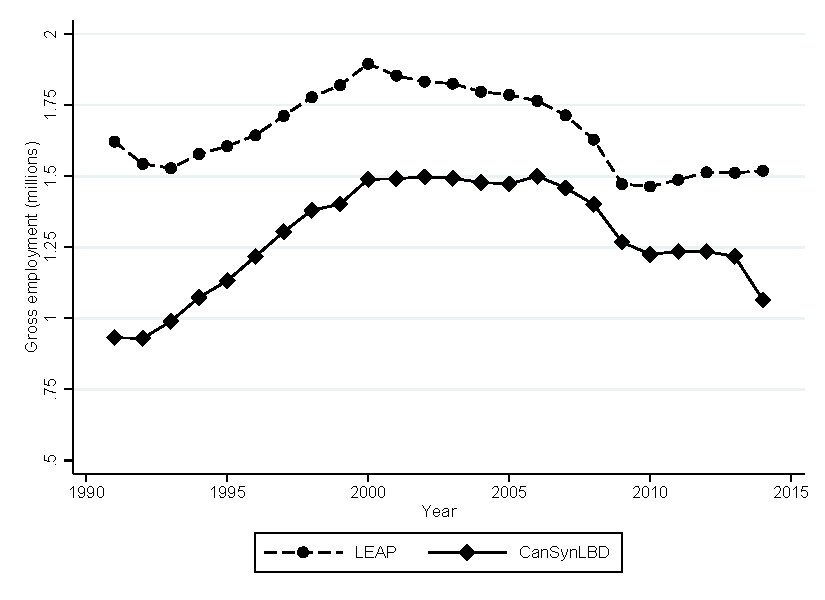
\includegraphics[height=2.8in, width=.7\linewidth]{graphs/Gross_employment_level_by_year_manufacturing_bw.pdf} 
\begin{minipage}{0.85\textwidth}
{\footnotesize Note: \TableNote  \par}
\end{minipage}
\end{figure}


\begin{figure} [H]
\centering
\caption{Total payroll by year (private)} \label{TotalPayrollPrivate}
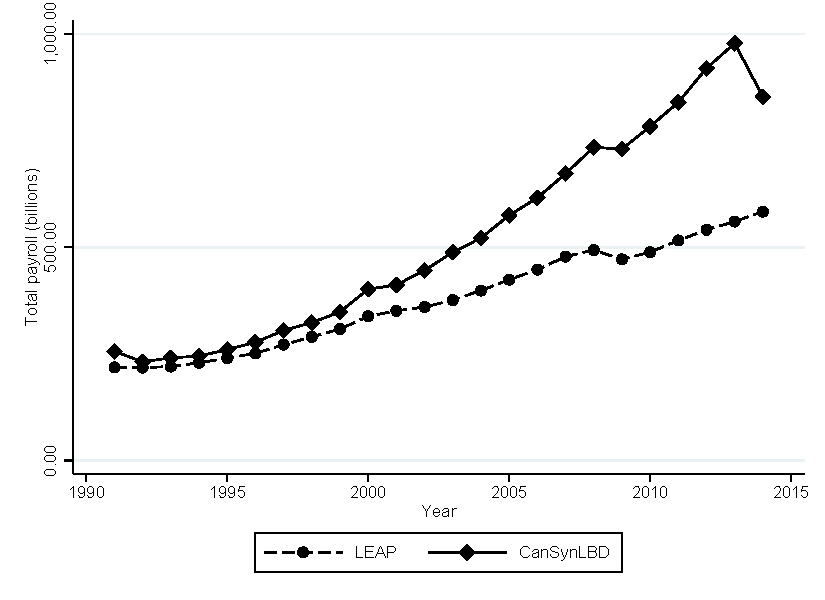
\includegraphics[height=2.8in, width=.7\linewidth]{graphs/Total_payroll_by_year_private_bw.pdf} 
\begin{minipage}{0.85\textwidth}
{\footnotesize Note: \TableNote \par}
\end{minipage}
\end{figure}
\begin{figure} [H]
\centering
\caption{Total payroll by year (manufacturing)} \label{TotalPayrollManufacturing}
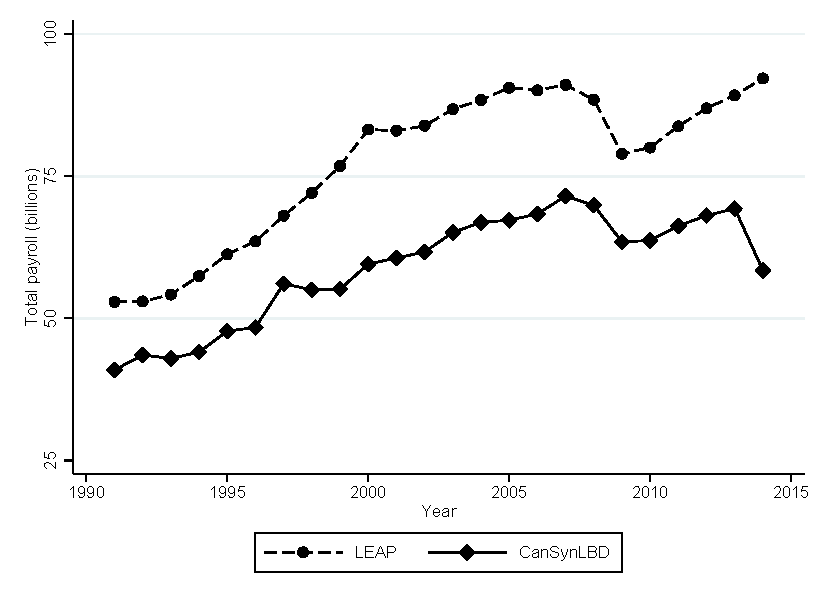
\includegraphics[height=2.8in, width=.7\linewidth]{graphs/Total_payroll_by_year_manufacturing_bw.pdf} 
\begin{minipage}{0.85\textwidth}
{\footnotesize Note: \TableNote \par}
\end{minipage}
\end{figure}

Figures \ref{FirmSharePrivate} and \ref{FirmShareManufacturing} plot the share of firms by two-digit industry and year for both the CanSynLBD and the LEAP databaseand show that those shares clustering along the 45-degree line.

\begin{figure} [H]
\centering
\caption{Share of firms by NAICS two-digit and year (private)} \label{FirmSharePrivate}
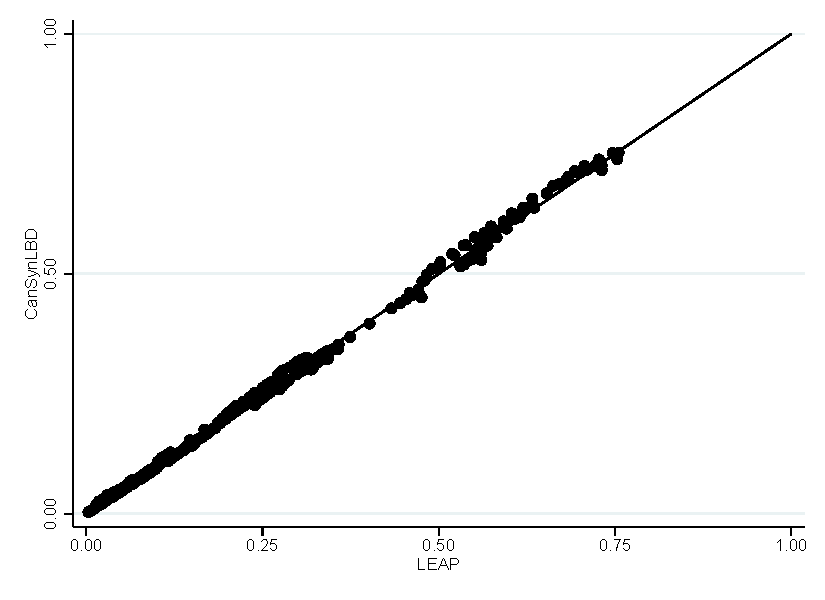
\includegraphics[height=2.8in, width=.7\linewidth]{graphs/Share_of_firms_by_NAICS_two-digit_and_year_private_bw.pdf} 
\begin{minipage}{0.85\textwidth}
{\footnotesize Note: \TableNote \par}
\end{minipage}
\end{figure}


\vspace{-15.5pt}
\begin{figure} [H]
\centering
\caption{Share of firms by NAICS two-digit and year (manufacturing)} \label{FirmShareManufacturing}
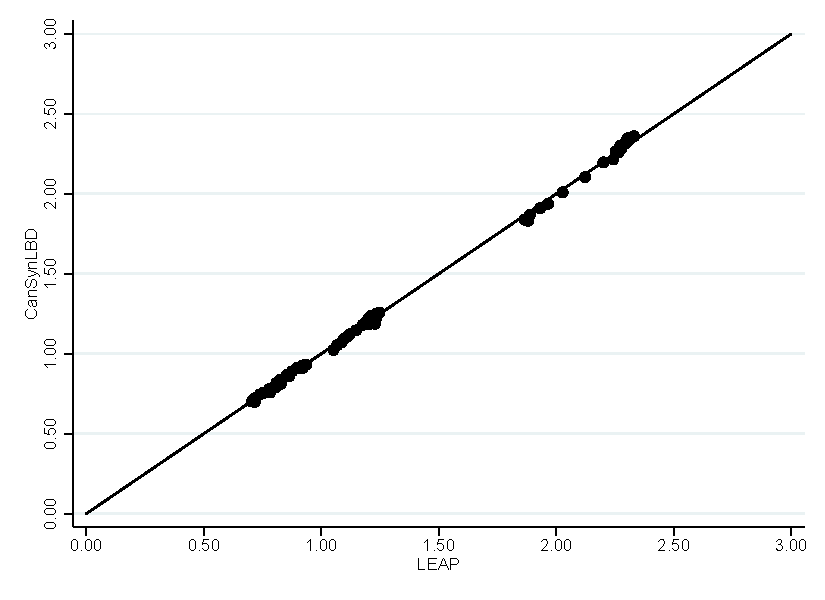
\includegraphics[height=2.8in, width=.7\linewidth]{graphs/Share_of_firms_by_NAICS_two-digit_and_year_Manufacturing_bw.pdf} 
\begin{minipage}{0.85\textwidth}
{\footnotesize Note: \TableNote \par}
\end{minipage}
\end{figure}

Figures \ref{EmploymentSharePrivate} and \ref{EmploymentShareManufacturing} plot the share of employment by two-digit industry and year for both the CanSynLBD and the LEAP database
\footnote{We define the share of employment as $x_{its} = X_{its}/\sum_{i} \sum_{t} X_{its}$, where $i$ are two-digit NAICS industries, $t$ are the years in-sample, $s$ indicates whether it is in the synthetic or confidential data, and $X_{its}$ is the total employment for industry $i$ and year $t$ for either the synthetic or confidential data $s$.} and show that those shares do not cluster along the 45-degree line. However, this hides significant differences between sectors as, for the share of employment for the manufacturing sector, we do observe more clustering along the 45-degrees.
\begin{figure} [H]
\centering
\caption{Share of employment by NAICS two-digit and year (private)} \label{EmploymentSharePrivate}
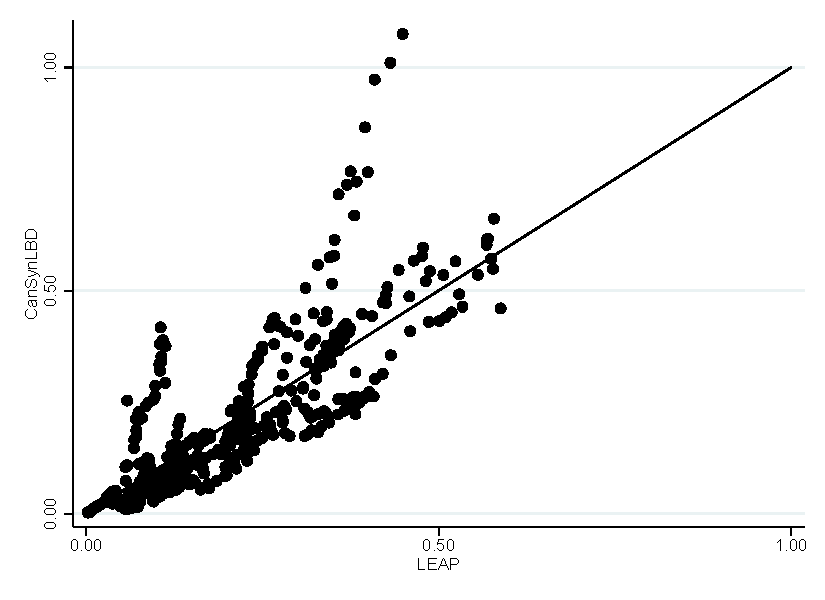
\includegraphics[height=2.8in, width=.7\linewidth]{graphs/Share_of_employment_by_NAICS_two-digit_and_year_private_bw.pdf} 
\begin{minipage}{0.85\textwidth}
{\footnotesize Note: \TableNote \par}
\end{minipage}
\end{figure}
\vspace{-15.5pt}
\begin{figure} [H]
\centering
\caption{Share of employment by NAICS two-digit and year (manufacturing)} \label{EmploymentShareManufacturing}
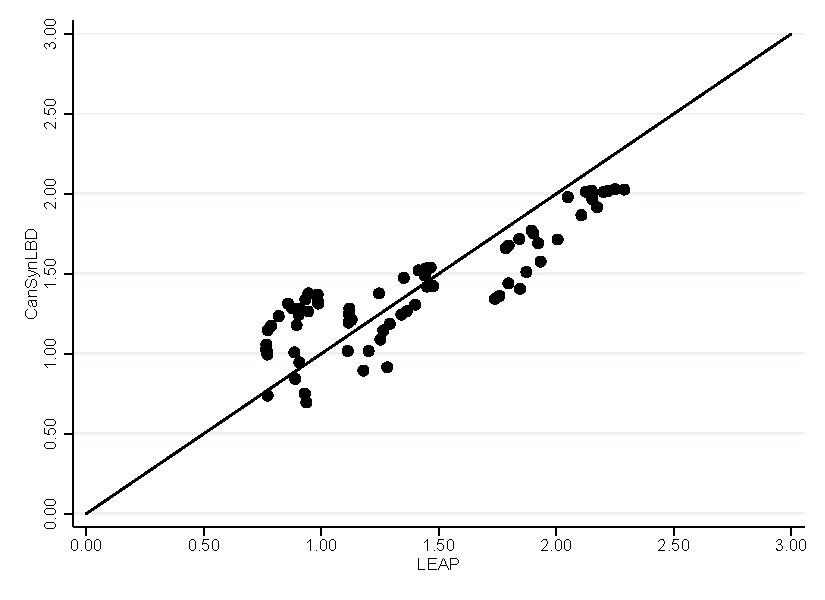
\includegraphics[height=2.8in, width=.7\linewidth]{graphs/Share_of_employment_by_NAICS_two-digit_and_year_Manufacturing_bw.pdf} 
\begin{minipage}{0.85\textwidth}
{\footnotesize Note: \TableNote \par}
\end{minipage}
\end{figure}

Figures \ref{PayrollSharePrivate} and \ref{PayrollShareManufacturing} plot the share of payroll by two-digit industry and year for both CanSynLBD and LEAP database and show that those shares do not cluster along the 45-degree line. Again, we do notice that for the share of employment for the manufacturing sector, we do observe more clustering along the 45-degrees.
\begin{figure} [H]
\centering
\caption{Share of payroll by NAICS two-digit and year (private)} \label{PayrollSharePrivate}
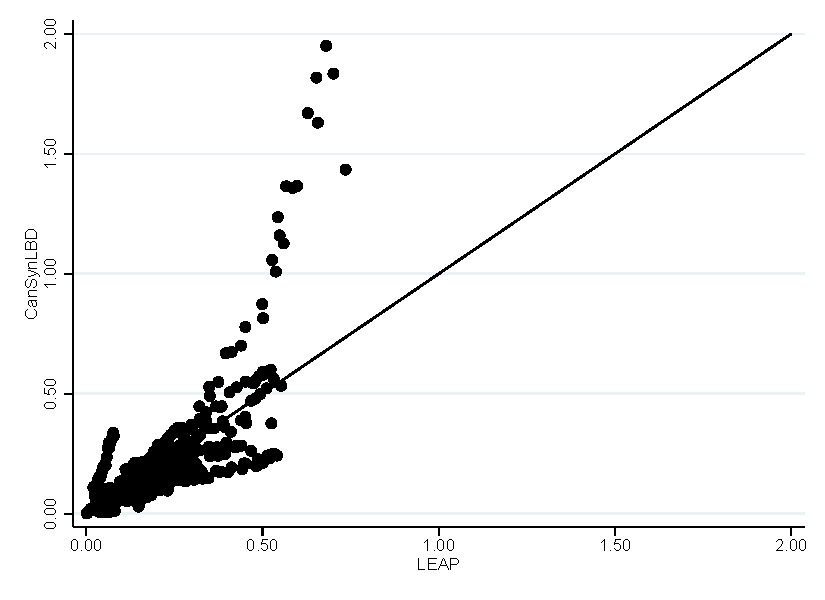
\includegraphics[height=2.8in, width=.7\linewidth]{graphs/Share_of_payroll_by_NAICS_two-digit_and_year_private_bw.pdf} 
\begin{minipage}{0.85\textwidth}
{\footnotesize Note: \TableNote \par}
\end{minipage}
\end{figure}
\vspace{-15.5pt}
\begin{figure} [H]
\centering
\caption{Share of payroll by NAICS two-digit and year (manufacturing)} \label{PayrollShareManufacturing}
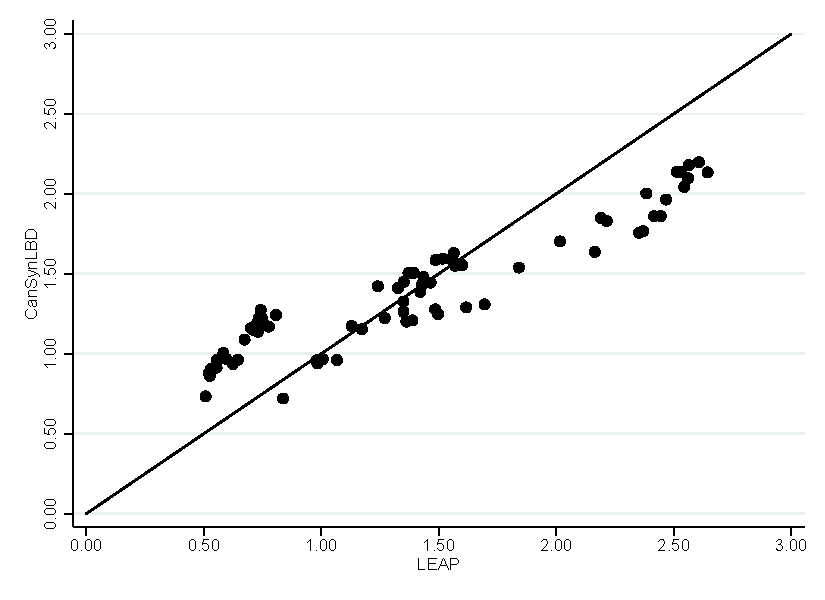
\includegraphics[height=2.8in, width=.7\linewidth]{graphs/Share_of_payroll_by_NAICS_two-digit_and_year_Manufacturing_bw.pdf} 
\begin{minipage}{0.85\textwidth}
{\footnotesize Note: \TableNote \par}
\end{minipage}
\end{figure}

\subsection{Firm Dynamics}
To assess how well the CanSynLBD captures firm dynamics, we also compute entry and exit rates of the private sector by year. Table \ref{FirmDynamics} shows that those rates for CanSynLBD are similar to LEAP database. To show further those rates are similar, we compute the divergence of entry rate as the entry rate of CanSynLBD net the entry rate of LEAP as well as the divergence of exit rate as the exit rate of CanSynLBD net the exit rate of LEAP (see Figure \ref{Divergence}).

\begin{table}[H]
  \centering
\begin{threeparttable}
 \caption{Entry and exit rates by year} \label{FirmDynamics} \medskip
\renewcommand{\arraystretch}{1}
\begin{tabular}{l|c c| c c| c c}
\toprule
&\multicolumn{2}{c|}{\textbf{LEAP}} &  \multicolumn{2}{c|}{\textbf{CanSynLBD}}&  \multicolumn{2}{c}{\textbf{Divergence}}\\
\textbf{Year}&\textbf{Entry Rate}&\textbf{Exit Rate}&\textbf{Entry Rate}&\textbf{Exit Rate} &\textbf{Entry Rate}&\textbf{Exit Rate}\\
\midrule
1992&11.77&11.72&11.16&11.71&-0.60&-0.00\\
1993&11.81&11.61&10.84&12.18&-0.97&0.57\\
1994&12.04&11.79&11.57&12.01&-0.47&0.22\\
1995&11.94&12.09&11.69&12.26&-0.25&0.17\\
1996&12.91&10.31&12.62&10.64&-0.29&0.32\\
1997&13.18&9.75&13.03&10.21&-0.15&0.47\\
1998&12.48&10.89&12.97&10.13&0.50&-0.75\\
1999&12.00&10.66&12.16&9.97&0.16&-0.69\\
2000&11.80&10.51&11.59&9.70&-0.20&-0.82\\
2001&11.44&10.20&11.33&9.52&-0.12&-0.68\\
2002&11.39&9.91&11.10&9.03&-0.29&-0.89\\
2003&11.17&10.21&10.52&9.37&-0.65&-0.84\\
2004&12.13&9.76&10.94&9.57&-1.20&-0.20\\
2005&11.92&10.07&11.07&9.86&-0.84&-0.21\\
2006&11.81&9.96&11.15&9.34&-0.66&-0.62\\
2007&12.28&9.80&10.99&9.31&-1.29&-0.49\\
2008&11.60&10.14&10.78&9.75&-0.82&-0.40\\
2009&10.77&9.93&9.99&9.81&-0.78&-0.12\\
2010&10.80&9.75&9.91&9.65&-0.89&-0.10\\
2011&10.62&9.79&9.73&10.00&-0.89&0.21\\
2012&10.60&9.76&10.02&10.20&-0.58&0.44\\
2013&10.16&9.71&9.95&10.32&-0.21&0.62\\
2014&9.93&10.11&9.26&10.70&-0.67&0.59\\

   \bottomrule
  \end{tabular} 
\begin{tablenotes}
\small
\item Note: \TableNote  We calculate the divergence of entry rate as the entry rate of CanSynLBD net the entry rate of LEAP and the divergence of exit rate as the exit rate of CanSynLBD net the exit rate of LEAP.
 \end{tablenotes}
 \end{threeparttable}
\end{table}

\begin{figure} [H]
\centering
\caption{Divergence of exit and entry rate between LEAP and CanSynLBD} \label{Divergence}
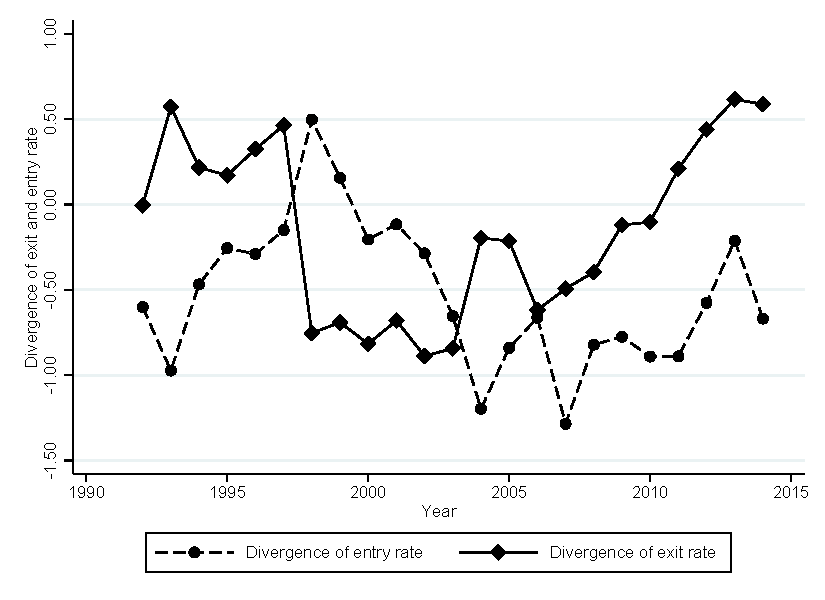
\includegraphics[height=2.8in, width=.7\linewidth]{graphs/Divergence_of_exit_and_entry_rate_between_LEAP_and_CanSynLBD_bw.pdf} 
\begin{minipage}{0.85\textwidth}
{\footnotesize Note: \TableNote  We calculate the divergence of entry rate as the entry rate of CanSynLBD net the entry rate of LEAP and the divergence of exit rate as the exit rate of CanSynLBD net the exit rate of LEAP. \par}
\end{minipage}
\end{figure}

\subsection{Dynamics of Job Flows}

One of the most important applications of LEAP is to generate statistics that describe job flows. Following \cite{DavisHaltiwangerSchuh}, the job creation is defined as the sum of all employment gains from expanding firms from year $t-1$ to year $t$ including entry firms. The job destruction rate is defined as the sum of all employment losses from contracting firms from year $t-1$ to year $t$ including exiting firms. Net job creation is the job creation rate minus the job destruction rate. Figures \ref{JobCreationPrivate} and \ref{JobCreationManufacturing} show the job creation rates from the CanSynLBD compared againg those of the LEAP. These figures show that the manufacturing sector has closer pattern than the private sector. We find a similar patterns for net job creation rates (Figures \ref{NetJobCreationPrivate} and  \ref{NetJobCreationManufacturing}).

\begin{figure} [H]
\centering
\caption{Job creation rate by year (private)} \label{JobCreationPrivate}
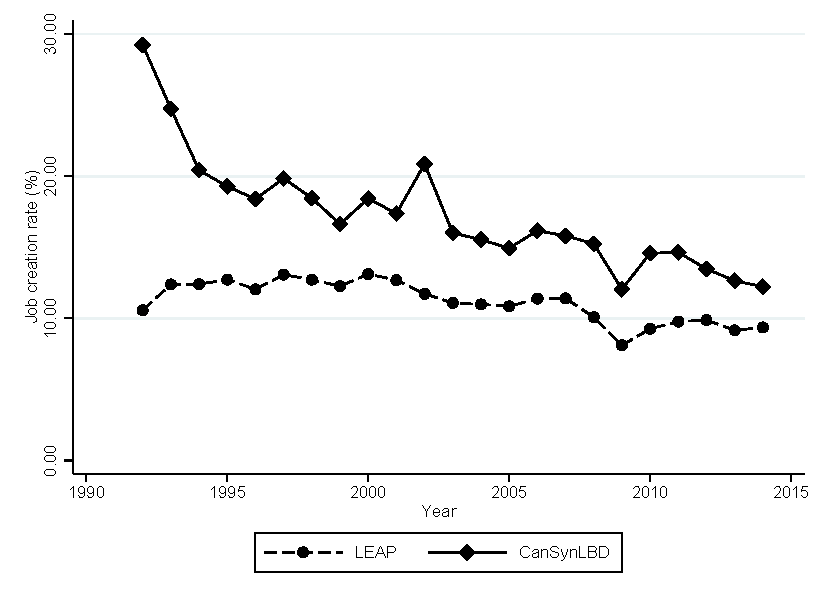
\includegraphics[height=2.8in, width=.7\linewidth]{graphs/Job_creation_rate_by_year_private_bw.pdf} 
\begin{minipage}{0.85\textwidth}
{\footnotesize Note: \TableNote \par}
\end{minipage}
\end{figure}

\begin{figure} [H]
\centering
\caption{Job creation rate  by year (manufacturing)} \label{JobCreationManufacturing}
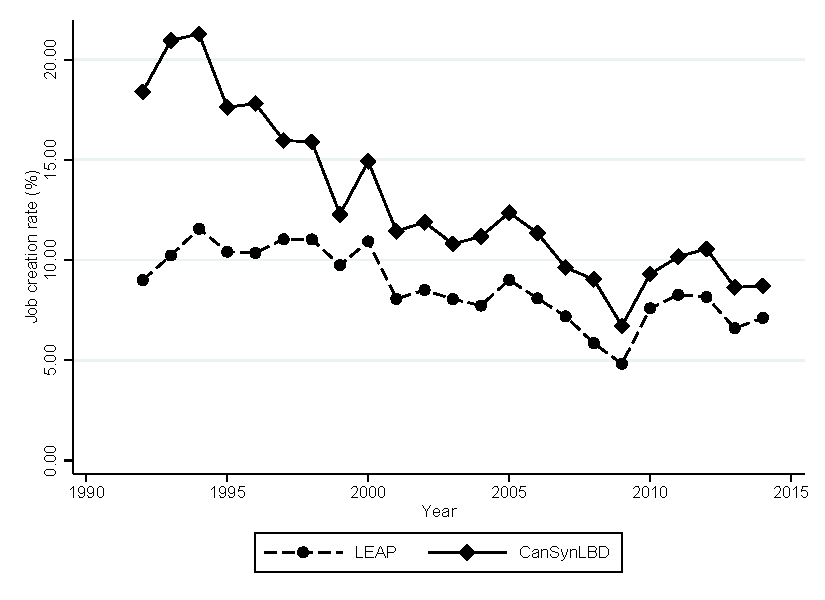
\includegraphics[height=2.8in, width=.7\linewidth]{graphs/Job_creation_rate_by_year_Manufacturing_bw.pdf} 
\begin{minipage}{0.85\textwidth}
{\footnotesize Note: \TableNote \par}
\end{minipage}
\end{figure}

\todo{LV regraph, dropping last year} \todo{JA: Should we mention this in the text including reasons if we drop the last year here?}
\begin{figure} [H]
\centering
\caption{Net job creation rate by year (private)} \label{NetJobCreationPrivate}
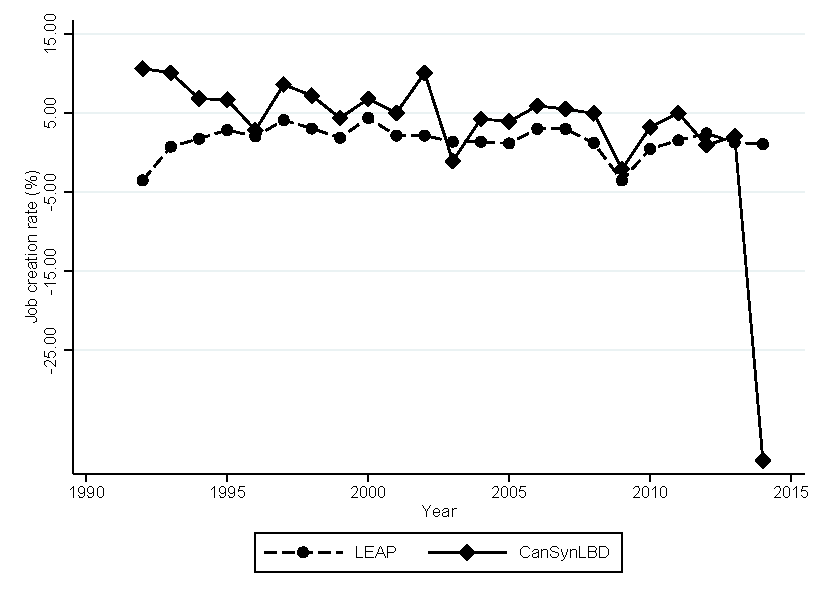
\includegraphics[height=2.8in, width=.7\linewidth]{graphs/Net_job_creation_rate_by_year_private_bw.pdf} 
\begin{minipage}{0.85\textwidth}
{\footnotesize Note: \TableNote \par}
\end{minipage}
\end{figure}
\begin{figure} [H]
\centering
\caption{Net job creation rate  by year (manufacturing)} \label{NetJobCreationManufacturing}
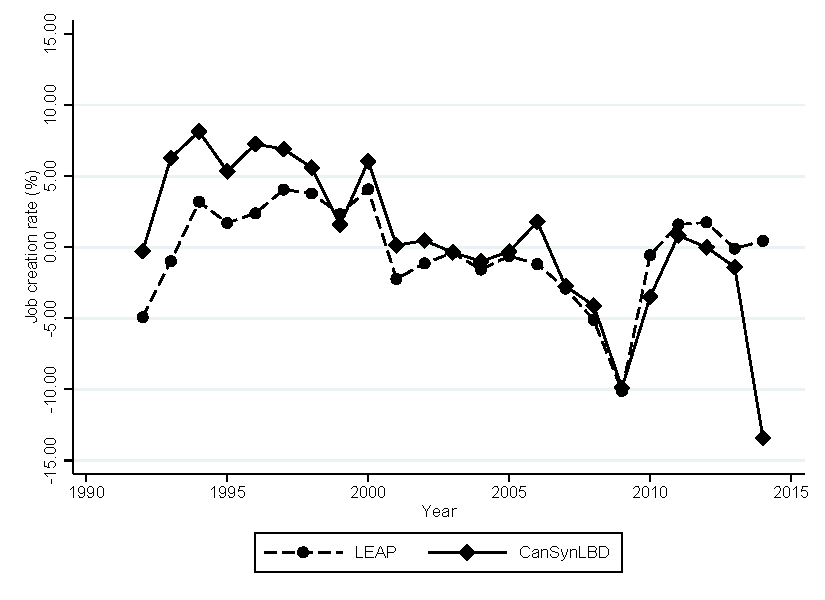
\includegraphics[height=2.8in, width=.7\linewidth]{graphs/Net_job_creation_rate_by_year_Manufacturing_bw.pdf} 
\begin{minipage}{0.85\textwidth}
{\footnotesize Note: $LEAP$ is the Longitudinal Employment Analysis Program and $CanSynLBD$ is the Canadian synthetic database based on LEAP. In this graph, we use 2015 vintage of LEAP for the manufacturing sector and drop last year observation of each firm. \par}
\end{minipage}
\end{figure}

\subsection{pMSE}

To compare the quality of the synthetic data relative to the confidential data, we compute $pMSE$, which is the mean-squared error of the predicted probabilities (i.e., propensity scores) for those two databases. Specifically, $pMSE$ is a metric to assess how well we are able to discern the high distributional similarity between synthetic data and confidential data. 

We follow the method by \textcite{SnokeSlavkovic2018} to calculate the $pMSE$. This method involved the following steps: 
\begin{enumerate}
    \item Append the $n_1$ rows of the confidential database $X$ to the $n_2$ rows of the synthetic database $X^s$ to create $X^{comb}$ with $N=n_1 + n_2$ rows.
    \item Create an indicator variable, $I$, to $X^{comb}$ subject to $I=\{1: X^{comb} \in X^s\}$. This means that we create an indicator variable of $1$ for the synthetic database and $0$ for the confidential database. 
    \item Fit the following model to predict $I$
    \begin{eqnarray}	
        I & = &\alpha + ALU_{it} + \lambda Pay_{it} + Age_{it}^{T}\beta + \lambda_t + \alpha_s + \epsilon_{it} \label{pMSE}
     \end{eqnarray}
     \todo{BD: I don't understand why the dependant variable has no indices?}
     \todo{JA: This is an indicator variable of $1$ for the synthetic database and $0$ for the confidential database. In this case, we need to add one more index in all variables as well.}
    where $ALU_{it}$ is the logarithm of average labour unit (ALU) of firm $i$ in year $t$, $Pay_{it}$ is the logarithm of payroll of firm $i$ in year $t$, $Age_{it}$ is a vector of dummy variables for age of firm $i$ in year $t$, $\lambda_t$ is the year fixed effect, $\alpha_s$ is an unobserved time-invariant industry-specific effect, and $\epsilon_{it}$ is the disturbance term of firm $i$ in year $t$. 
    \item calculate the predicted probabilities, $\hat{p}_i$ for each row of $X^{comb}$
    \item Compute the $pMSE=\frac{1}{N}\sum_{i=1}^N(\hat{p}_i - 0.5)^2$
\end{enumerate}
A $pMSE$ = 0 means every $\hat{p}_i = 0.5$. 

To compute the $pMSE$, we estimate equation \ref{pMSE} using both the logit and probit models. Table \ref{pMSE_regression} \todo{BD: Are those coefficients or marginal effects? Does it make sense to show coefficients? Or are we interested only in the last row? If we are interested in the coefficient, why is there no discussion of those?} \todo{Those are coefficients. I think we are interested in the last row.} shows the calculated value of $pMSE$, which is lower for the manufacturing sector than the public sector in both regressions. This is because, as we explained before, the synthetic data mirrors the original data more closely in the case of the manufacturing sector.

\begin{table}[H]
  \centering
\begin{threeparttable}
 \caption{pMSE estimates} \label{pMSE_regression} \medskip
\renewcommand{\arraystretch}{1}
\begin{tabular}{l|c c| c c}
\toprule
\textbf{Independent Variables}&\multicolumn{2}{c|}{\textbf{Logistic Regression}} &  \multicolumn{2}{c}{\textbf{Probit Regression}}\\
\midrule
          &\multicolumn{1}{c}{Manufacturing}&\multicolumn{1}{c}{Private}&\multicolumn{1}{c}{Manufacturing}&\multicolumn{1}{c}{Private}\\
\hline
Ln ALU    &   0.1580\sym{***}&   0.7138\sym{***}&   0.1003\sym{***}&   0.4390\sym{***}\\
          & (0.0039)         & (0.0010)         & (0.0024)         & (0.0006)         \\
[1em]
Ln Pay    &   0.0039         &  -0.4426\sym{***}&   0.0012         &  -0.2691\sym{***}\\
          & (0.0037)         & (0.0010)         & (0.0023)         & (0.0006)         \\
[1em]
Age 3-4   &   0.0392\sym{***}&   0.0972\sym{***}&   0.0252\sym{***}&   0.0618\sym{***}\\
          & (0.0078)         & (0.0017)         & (0.0049)         & (0.0010)         \\
[1em]
Age 5-7   &  -0.0382\sym{***}&   0.0477\sym{***}&  -0.0233\sym{***}&   0.0309\sym{***}\\
          & (0.0073)         & (0.0016)         & (0.0045)         & (0.0010)         \\
[1em]
Age 8-12  &  -0.1258\sym{***}&  -0.0263\sym{***}&  -0.0781\sym{***}&  -0.0152\sym{***}\\
          & (0.0071)         & (0.0015)         & (0.0044)         & (0.0009)         \\
[1em]
Age 13 or more&  -0.2190\sym{***}&  -0.1024\sym{***}&  -0.1365\sym{***}&  -0.0627\sym{***}\\
          & (0.0074)         & (0.0016)         & (0.0046)         & (0.0010)         \\
\hline
\(N\)     &  2243011         & 34638723         &  2243011         & 34638723         \\
pseudo \(R^{2}\)&   0.0112         &   0.0318         &   0.0112         &   0.0320         \\
pMSE      &   0.0041         &   0.0121         &   0.0041         &   0.0124         \\

   \bottomrule
  \end{tabular} 
\begin{tablenotes}
\small
\item Note: An observation is a firm and a year of both synthetic and original databases. In all specifications, we include both time and industry fixed effects. Standard errors are in parentheses. In this table, we use 2015 vintage of LEAP to create the synthetic database and drop last year observation of each firm. ***, **, and * indicate statistically significant coefficients at 1\%, 5\%, and 10\% percent levels, respectively.
 \end{tablenotes}
 \end{threeparttable}
\end{table}

\subsection{Regression Analysis}

To assess how well the CanSynLBD captures variability in economic growth due to industry and firm age, we estimate the following dynamic panel data model:
\begin{eqnarray}	
ALU_{it} & = & \alpha + \theta ALU_{i,t-1} + \lambda Pay_{it} + Age_{it}^{T}\beta + \lambda_t + \alpha_s + \epsilon_{it}
\end{eqnarray}
where $ALU_{it}$ is the logarithm of average labour unit (ALU) of firm $i$ in year $t$, $ALU_{i,t-1}$ is the logarithm of last year's average labour unit (ALU) of firm $i$, $Pay_{it}$ is the logarithm of payroll of firm $i$ in year $t$, $Age_{it}$ is a vector of dummy variables for age of firm $i$ in year $t$, $\lambda_t$ is the year fixed effect, $\alpha_s$ is an unobserved time-invariant industry-specific effect, and $\epsilon_{it}$ is the disturbance term of firm $i$ in year $t$. 

\begin{table}[H]
  \centering
\begin{threeparttable}
 \caption{Regression coefficients (OLS)} \label{OLS} \medskip
\renewcommand{\arraystretch}{1}
\begin{tabular}{l|c c| c c}
\toprule
\textbf{Independent Variables}&\multicolumn{2}{c|}{\textbf{LEAP}} &  \multicolumn{2}{c}{\textbf{CanSynLBD}}\\
\midrule
&\multicolumn{1}{c}{Private}&\multicolumn{1}{c}{Manufacturing}&\multicolumn{1}{c}{Private}&\multicolumn{1}{c}{Manufacturing}\\
\hline
AR(1) Coefficient&   0.2031\sym{***}&   0.2481\sym{***}&   0.3970\sym{***}&   0.4405\sym{***}\\
          & (0.0001)         & (0.0005)         & (0.0002)         & (0.0007)         \\
[1em]
Ln Pay    &   0.7847\sym{***}&   0.7300\sym{***}&   0.5481\sym{***}&   0.5228\sym{***}\\
          & (0.0001)         & (0.0005)         & (0.0002)         & (0.0006)         \\
[1em]
Age 3-4   &  -0.1202\sym{***}&  -0.1717\sym{***}&  -0.1223\sym{***}&  -0.2340\sym{***}\\
          & (0.0003)         & (0.0014)         & (0.0004)         & (0.0016)         \\
[1em]
Age 5-7   &  -0.1260\sym{***}&  -0.1891\sym{***}&  -0.1235\sym{***}&  -0.2507\sym{***}\\
          & (0.0003)         & (0.0014)         & (0.0004)         & (0.0016)         \\
[1em]
Age 8-12  &  -0.1268\sym{***}&  -0.1973\sym{***}&  -0.1169\sym{***}&  -0.2551\sym{***}\\
          & (0.0003)         & (0.0013)         & (0.0004)         & (0.0016)         \\
[1em]
Age 13 or more&  -0.1246\sym{***}&  -0.1992\sym{***}&  -0.1101\sym{***}&  -0.2577\sym{***}\\
          & (0.0003)         & (0.0014)         & (0.0004)         & (0.0017)         \\
\hline
\(N\)     & 15708195         &  1015293         & 13573225         &   959764         \\
\(R^{2}\) &   0.9696         &   0.9743         &   0.9444         &   0.9523         \\

   \bottomrule
  \end{tabular} 
\begin{tablenotes}
\small
\item Note: In all specifications, we include both year and industry fixed effects. Standard errors are in parentheses. $LEAP$ is the Longitudinal Employment Analysis Program and $CanSynLBD$ is the Canadian synthetic database based on LEAP. In this table, we use the 2015 vintage of LEAP and drop last year observation of each firm. ***, **, and * indicate statistically significant coefficients at 1\%, 5\%, and 10\% percent levels, respectively.
 \end{tablenotes}
 \end{threeparttable}
\end{table}

We estimate the model separately on LEAP and CanSynLBD data for the private and manufacturing sectors and find that the CansynLBD data provides similar predictions to LEAP data (Tables  \ref{OLS}).\todo{compute overlap interval} \todo{JA: @Lars, I think you mentioned once that you would like to calculate this. I could calculate using the method explained in the appendix.}

\begin{table}[H]
  \centering
\begin{threeparttable}
 \caption{Regression coefficients (Dynamic)} \label{Dynamic - GMM} \medskip
\renewcommand{\arraystretch}{1}
\begin{tabular}{l|c c| c c}
\toprule
\textbf{Independent Variables}&\multicolumn{2}{c|}{\textbf{LEAP}} &  \multicolumn{2}{c}{\textbf{CanSynLBD}}\\
\midrule
&\multicolumn{1}{c}{Private}&\multicolumn{1}{c}{Manufacturing}&\multicolumn{1}{c}{Private}&\multicolumn{1}{c}{Manufacturing}\\
\hline
AR(1) Coefficient&   0.0805\sym{***}&   0.1189\sym{***}&   0.5722\sym{***}&   0.5425\sym{***}\\
          & (0.0003)         & (0.0018)         & (0.0024)         & (0.0084)         \\
[1em]
Ln Pay    &   0.8991\sym{***}&   0.8523\sym{***}&   0.4101\sym{***}&   0.4302\sym{***}\\
          & (0.0002)         & (0.0015)         & (0.0018)         & (0.0067)         \\
[1em]
Age 3-4   &  -0.0450\sym{***}&  -0.0797\sym{***}&  -0.2075\sym{***}&  -0.2972\sym{***}\\
          & (0.0002)         & (0.0014)         & (0.0010)         & (0.0051)         \\
[1em]
Age 5-7   &  -0.0438\sym{***}&  -0.0860\sym{***}&  -0.2129\sym{***}&  -0.3162\sym{***}\\
          & (0.0002)         & (0.0015)         & (0.0011)         & (0.0059)         \\
[1em]
Age 8-12  &  -0.0418\sym{***}&  -0.0923\sym{***}&  -0.2187\sym{***}&  -0.3294\sym{***}\\
          & (0.0003)         & (0.0017)         & (0.0013)         & (0.0070)         \\
[1em]
Age 13 or more&  -0.0379\sym{***}&  -0.0898\sym{***}&  -0.2318\sym{***}&  -0.3414\sym{***}\\
          & (0.0003)         & (0.0019)         & (0.0015)         & (0.0080)         \\
\hline
\(N\)     & 15708195         &  1015293         & 13573225         &   959764         \\
m2        & -14.5000         &  -2.2200         & -27.5400         &  -9.4400         \\
Sargan test&  6.9e+04         &  4.6e+03         &  1.5e+04         &  1.5e+03         \\
df of Sargan Test& 252.0000         & 252.0000         & 252.0000         & 252.0000         \\
P value of Sargan test&   0.0000         &   0.0000         &   0.0000         &   0.0000         \\

   \bottomrule
  \end{tabular} 
\begin{tablenotes}
\small
\item Note: In this table, $m2$ is the Arellano-Bond test for zero autocorrelation in first-differenced errors for order two. $LEAP$ is the Longitudinal Employment Analysis Program and $CanSynLBD$ is the Canadian synthetic database based on LEAP. In this graph, we use the 2015 vintage of LEAP and drop last year observation of each firm. Standard errors are in parentheses. ***, **, and * indicate statistically significant coefficients at 1\%, 5\%, and 10\% percent levels, respectively.
 \end{tablenotes}
 \end{threeparttable}
\end{table}

As $ALU_{st-1}$ is correlated with $\alpha_{s}$ because $ALU_{st-1}$ is a function of $\alpha_{s}$, OLS estimators are biased and inconsistent. 
To take this endogeneity bias into account, we use the estimation method from \textcite{RePEc:oup:restud:v:58:y:1991:i:2:p:277-297.} and find similar predictions (Table \ref{Dynamic - GMM}). To check the validity of the model, we use two tests. First, to test for autocorrelation, we use the test $m2$ by \textcite{RePEc:oup:restud:v:58:y:1991:i:2:p:277-297.}. In the table, we report the $z$ test statistic for $m2$ test for zero autocorrelation in the  first-differenced errors of order two. Second, we use the Sargan test to verify the validity of instrument subsets (showned in the last three rows in the table).

We furthermore estimate the model using the system GMM  method proposed by \textcite{RePEc:eee:econom:v:68:y:1995:i:1:p:29-51} and \textcite{RePEc:eee:econom:v:87:y:1998:i:1:p:115-143} and find similar predictions as before (Table \ref{Dynamic - system GMM}). 

\begin{table}[H]
  \centering
\begin{threeparttable}
 \caption{Regression coefficients (Dynamic - system GMM)} \label{Dynamic - system GMM} \medskip
\renewcommand{\arraystretch}{1}
\begin{tabular}{l|c c| c c}
\toprule
\textbf{Independent Variables}&\multicolumn{2}{c|}{\textbf{LEAP}} &  \multicolumn{2}{c}{\textbf{CanSynLBD}}\\
\midrule
&\multicolumn{1}{c}{Private}&\multicolumn{1}{c}{Manufacturing}&\multicolumn{1}{c}{Private}&\multicolumn{1}{c}{Manufacturing}\\
\hline
AR(1) Coefficient&   0.0978\sym{***}&   0.1614\sym{***}&   0.5111\sym{***}&   0.5780\sym{***}\\
          & (0.0002)         & (0.0014)         & (0.0008)         & (0.0041)         \\
[1em]
Ln Pay    &   0.8854\sym{***}&   0.8161\sym{***}&   0.4562\sym{***}&   0.4022\sym{***}\\
          & (0.0002)         & (0.0012)         & (0.0006)         & (0.0033)         \\
[1em]
Age 3-4   &  -0.0555\sym{***}&  -0.1097\sym{***}&  -0.1828\sym{***}&  -0.3177\sym{***}\\
          & (0.0002)         & (0.0012)         & (0.0004)         & (0.0028)         \\
[1em]
Age 5-7   &  -0.0558\sym{***}&  -0.1201\sym{***}&  -0.1860\sym{***}&  -0.3408\sym{***}\\
          & (0.0002)         & (0.0013)         & (0.0005)         & (0.0031)         \\
[1em]
Age 8-12  &  -0.0548\sym{***}&  -0.1298\sym{***}&  -0.1875\sym{***}&  -0.3583\sym{***}\\
          & (0.0002)         & (0.0014)         & (0.0005)         & (0.0036)         \\
[1em]
Age 13 or more&  -0.0524\sym{***}&  -0.1317\sym{***}&  -0.1943\sym{***}&  -0.3747\sym{***}\\
          & (0.0002)         & (0.0016)         & (0.0006)         & (0.0041)         \\
\hline
\(N\)     & 15708195         &  1015293         & 13573225         &   959764         \\
m2        & -11.4300         &   1.3900         & -41.6000         &  -7.6700         \\
Sargan test&  7.7e+04         &  6.3e+03         &  1.8e+04         &  1.7e+03         \\
df of Sargan Test& 274.0000         & 274.0000         & 274.0000         & 274.0000         \\
P value of Sargan test&   0.0000         &   0.0000         &   0.0000         &   0.0000         \\

   \bottomrule
  \end{tabular} 
\begin{tablenotes}
\small
\item Note: An observation is a firm and a year. In this table, $m2$ is the Arellano-Bond test for zero autocorrelation in first-differenced errors for order two. $LEAP$ is the Longitudinal Employment Analysis Program and $CanSynLBD$ is the Canadian synthetic database based on LEAP. In this table, we use 2015 vintage of LEAP and drop last year observation of each firm. Standard errors are in parentheses. ***, **, and * indicate statistically significant coefficients at 1\%, 5\%, and 10\% percent levels, respectively.
 \end{tablenotes}
 \end{threeparttable}
\end{table}

We also estimate above dynamic panel data model with a first-order moving average using appropriate instruments for both level and difference equation as proposed by \textcite{RePEc:eee:econom:v:68:y:1995:i:1:p:29-51} and \textcite{RePEc:eee:econom:v:87:y:1998:i:1:p:115-143}:
\begin{eqnarray}	
ALU_{it}&=&\alpha +\theta ALU_{i,t-1}+\lambda Pay_{it}+Age_{it}^{T}\beta+\lambda_t+\alpha_s+\epsilon_{it}+\gamma\epsilon_{it-1}
\end{eqnarray}

Table \ref{Dynamic - system GMM with MA(1)} shows that the CansynLBD provides similar predictions to the LEAP.

\begin{table}[H]
  \centering
\begin{threeparttable}
 \caption{Regression coefficients (Dynamic - system GMM with MA(1))} \label{Dynamic - system GMM with MA(1)} \medskip
\renewcommand{\arraystretch}{1}
\begin{tabular}{l|c c| c c}
\toprule
\textbf{Independent Variables}&\multicolumn{2}{c|}{\textbf{LEAP}} &  \multicolumn{2}{c}{\textbf{CanSynLBD}}\\
\midrule
&\multicolumn{1}{c}{Private}&\multicolumn{1}{c}{Manufacturing}&\multicolumn{1}{c}{Private}&\multicolumn{1}{c}{Manufacturing}\\
\hline
AR(1) Coefficient&   0.2005\sym{***}&   0.2821\sym{***}&   0.4850\sym{***}&   0.5737\sym{***}\\
          & (0.0007)         & (0.0040)         & (0.0012)         & (0.0059)         \\
[1em]
Ln Pay    &   0.8044\sym{***}&   0.7135\sym{***}&   0.4760\sym{***}&   0.4056\sym{***}\\
          & (0.0005)         & (0.0034)         & (0.0009)         & (0.0046)         \\
[1em]
Age 3-4   &  -0.1245\sym{***}&  -0.2033\sym{***}&  -0.1716\sym{***}&  -0.3158\sym{***}\\
          & (0.0005)         & (0.0032)         & (0.0006)         & (0.0037)         \\
[1em]
Age 5-7   &  -0.1328\sym{***}&  -0.2264\sym{***}&  -0.1733\sym{***}&  -0.3389\sym{***}\\
          & (0.0005)         & (0.0035)         & (0.0006)         & (0.0043)         \\
[1em]
Age 8-12  &  -0.1383\sym{***}&  -0.2454\sym{***}&  -0.1731\sym{***}&  -0.3560\sym{***}\\
          & (0.0006)         & (0.0039)         & (0.0007)         & (0.0051)         \\
[1em]
Age 13 or more&  -0.1441\sym{***}&  -0.2586\sym{***}&  -0.1774\sym{***}&  -0.3717\sym{***}\\
          & (0.0006)         & (0.0042)         & (0.0008)         & (0.0058)         \\
\hline
\(N\)     & 15708195         &  1015293         & 13573225         &   959764         \\
m2        &   8.2000         &   7.0600         & -40.0300         &  -6.6400         \\
Sargan test&  2.8e+04         &  2.3e+03         &  1.7e+04         &  1.3e+03         \\
df of Sargan Test& 251.0000         & 251.0000         & 251.0000         & 251.0000         \\
P value of Sargan test&   0.0000         &   0.0000         &   0.0000         &   0.0000         \\

   \bottomrule
  \end{tabular} 
\begin{tablenotes}
\small
\item Note: An observation is a firm and a year. In this table, $m2$ is the Arellano-Bond test for zero autocorrelation in first-differenced errors for order two. $LEAP$ is the Longitudinal Employment Analysis Program and $CanSynLBD$ is the Canadian synthetic database based on LEAP. In this table, we use 2015 vintage of LEAP and drop last year observation of each firm. Standard errors are in parentheses. ***, **, and * indicate statistically significant coefficients at 1\%, 5\%, and 10\% percent levels, respectively.
 \end{tablenotes}
 \end{threeparttable}
\end{table}